\documentclass[a4paper]{oblivoir}
\usepackage{amsmath,amssymb,kotex,kswrapfig,mdframed,paralist,tabu}
\usepackage{fapapersize}
\usefapapersize{210mm,297mm,40mm,*,20mm,*}

\usepackage{tabto,pifont}
\TabPositions{0.2\textwidth,0.4\textwidth,0.6\textwidth,0.8\textwidth}
\newcommand\tabb[5]{\par\noindent
\ding{172}\:{\ensuremath{\displaystyle#1}}
\tab\ding{173}\:\:{\ensuremath{\displaystyle#2}}
\tab\ding{174}\:\:{\ensuremath{\displaystyle#3}}
\tab\ding{175}\:\:{\ensuremath{\displaystyle#4}}
\tab\ding{176}\:\:{\ensuremath{\displaystyle#5}}}

\usepackage{graphicx}

%\pagestyle{empty}

%%% Counters
\newcounter{num}
\counterwithout{subsection}{section}

%%% Commands
\newcommand\prob[1]
{\vs\bigskip\bigskip\par\noindent\stepcounter{num} \textbf{문제 \thenum) #1}\par\noindent}

\newcommand\pb[1]{\ensuremath{\fbox{\phantom{#1}}}}

\newcommand\ba{\ensuremath{\:|\:}}

\newcommand\vs[1]{\vspace{70pt}}

\newcommand\an[1]{\bigskip\par\noindent\textbf{문제 #1)}\par\noindent}

%%% Meta Commands
\let\oldsection\section
\renewcommand\section{\clearpage\oldsection}

\let\emph\textsf

\begin{document}
\begin{center}
\LARGE종현, 추가과제 08
\end{center}
\begin{flushright}
날짜 : 2017년 \(\pb3\)월 \(\pb{10}\)일 \(\pb{월}\)요일
,\qquad
제한시간 : \pb{17년}분
,\qquad
점수 : \pb{20} / \pb{20}
\end{flushright}

\setcounter{subsection}{4}
%%
\subsection{함수의 뜻과 그래프}
\vspace{-60pt}
% 함수 5-1
\prob{}
두 집합 \(X=\{-1,0,1\}\), \(Y=\{0,1,2,3\}\)에 대하여 다음 중 집합 \(X\)에서 \(Y\)로의 함수가 \underline{아닌} 것은?
\par\bigskip
\noindent\ding{172}\:\:{\(f(x)=x+1\)}
\tabto{0.5\textwidth}\ding{173}\:\:{\(f(x)=x^2+2\)}
\par\bigskip\medskip\noindent\ding{174}\:\:{\(f(x)=|x|\)}
\tabto{0.5\textwidth}\ding{175}\:\:{\(f(x)=\begin{cases}0&(x\le0)\\2&(x>0)\end{cases}\)}
\par\medskip\noindent\ding{176}\:\:{\(f(x)=\sqrt{1-x}\)}

% 함수 5-2
\prob{}
함수 \(f\)가 실수 전체의 집합에서
\[f(x)=\begin{cases}1-x&(x\text{는 유리수})\\1+x&(x\text{는 무리수})\end{cases}\]
로 정의될 때, \(f(2)+f(1-\sqrt2)\)의 값은?
\par\bigskip
\tabb{1-\sqrt2}{2-\sqrt2}{\sqrt2}2{2\sqrt2}

% 함수 5-3
\prob{}
집합 \(X=\{x\,|\,1\le x\le 7,\quad x\text{는 자연수}\}\)를 정의역으로 하는 함수 \(f\)에 대하여
\[f(x)=\begin{cases}2-x&(x\text{는 홀수})\\x-3&(x\text{는 짝수})\end{cases}\]
일 때, 함수 \(f\)의 치역의 모든 원소의 합은?
\par\bigskip
\tabb{-5}{-3}{-1}13

% 함수 5-4
\prob{}
집합 \(X=\{a,b\}\)에서 정의된 두 함수
\[f(x)=2x^2+4x-5,\qquad g(x)=x^2+3x+7\]
이 서로 같을 때, 서로 다른 두 실수 \(a\), \(b\)에 대하여 \(a+b\)의 값은?
\par\bigskip
\tabb{-2}{-1}012

% 함수 5-5
\prob{}
두 집합 \(X=\{x\,|\,-1\le x\le 5\}\), \(Y=\{y\,|\,-7\le y\le 5\}\)에 대하여 집합 \(X\)에서 집합 \(Y\)로의 함수 \(f(x)=ax+b\:(a>0)\)가 일대일대응일 때, \(f(3)\)의 값은?(단, \(a\), \(b\)는 실수이다.)
\par\bigskip
\tabb{-5}{-3}{-1}13

% 함수 5-6
\prob{}
집합 \(X=\{0,1,2,3\}\)에 대하여 \(X\)에서 \(X\)로의 함수 \(f(x)\), \(g(x)\), \(h(x)\)를 다음과 같이 정의한다.
\begin{align*}
f(x)&=\left[\frac{x^2}{10}\right]\\
g(x)&=\frac{|x+1|+|x-1|}2\\
h(x)&=(x\text{를 4로 나누었을 때의 나머지})
\end{align*}
일대일 함수의 개수를 \(a\), 항등함수의 개수를 \(b\), 상수함수의 개수를 \(c\)라고 할 때, \(a-2b+3c\)의 값은?
(단, \([x]\)는 \(x\)보다 크지 않은 최대의 정수이다.)
\par\bigskip
\tabb12345

% 함수 5-7
\prob{}
집합 \(X=\{-1,0,1\}\)에 대하여 \(X\)에서 \(X\)로의 함수 중 일대일대응의 개수를 \(p\), 항등함수의 개수를 \(q\), 상수함수의 개수를 \(r\)라고 할 때, \(p+q+r\)의 값은?
\par\bigskip
\tabb789{10}{11}


%%
\subsection{합성함수와 역함수}
\vspace{-60pt}

% 함수 6-1
\prob{}
\[f(x)=\begin{cases}12-4x&(x\ge2)\\4&(x<2)\end{cases},\quad g(x)=\frac14x^2-2\]
에 대하여 \((g\circ f)(1)+(f\circ g)(6)\)의 값은?
\par\bigskip
\tabb{-14}{-12}{-10}{-8}{-6}

% 함수 6-2
\prob{}
두 함수 \(f(x)=2x+k\), \(g(x)=-3x+4\)에 대하여 \(f\circ g=g\circ f\)일 때, \(f(3)\)의 값은?
(단, \(k\)는 상수이다.)
\par\bigskip
\tabb13579

% 함수 6-3
\prob{}
\begin{minipage}{.45\textwidth}
집합 \(X=\{1,2,3\}\)에 대하여 함수\\ \(f:X\to X\)의 대응관계는 다음과 같다.
\begin{align*}
f^1(x)&=f(x),\\
f^{n+1}(x)&=f(f^n(x))\\
&(n=1,2,3,\cdots)
\end{align*}
\end{minipage}
\begin{minipage}{.45\textwidth}
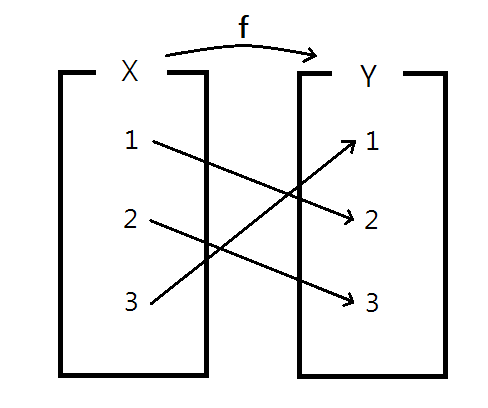
\includegraphics[width=0.9\textwidth]{a_function}
\end{minipage}
\par\noindent
이라고 할 때, \(f^{100}(1)-f^{200}(3)\)의 값은?
\par\bigskip
\tabb{-2}{-1}012

\newpage
% 함수 6-4
\prob{}
정의역과 공역이 실수 전체인 함수 \(f(x)\)가 다음과 같다.
\[f(x)=\begin{cases}x^2-1&(x\le0)\\(a-1)x+a^2-4&(x>0)\end{cases}\]
함수 \(f(x)\)의 역함수가 존재하도록 하는 상수 \(a\)의 값은?
\par\bigskip
\tabb{-\sqrt3}{-\sqrt2}0{\sqrt2}{\sqrt3}

% 함수 6-5
\prob{}
두 함수 \(f(x)=2x-1\), \(g(x)=-3x+5\)에 대하여 \((f\circ(f\circ g)^{-1}\circ f)(k)=5\)를 만족시키는 상수 \(k\)의 값은?
\par\bigskip
\tabb{-5}{-4}{-3}{-2}{-1}

% 함수 6-6
\prob{}
함수 \(f(x)=mx+n\)의 역함수가 \(f^{-1}(x)=\frac13x+\frac43\)일 때, 상수 \(m\), \(n\)에 대하여 \(m^2+n^2\)의 값은?
\par\bigskip
\tabb9{16}{25}{32}{41}

% 함수 6-7
\prob{}
함수 \(f(x)=x^2-2x+2\:(x\ge1)\)의 역함수를 \(f^{-1}(x)\)라고 할 때, 두 함수 \(y=f(x)\), \(y=f^{-1}(x)\)의 그래프의 두 교점 사이의 거리는?
\par\bigskip
\tabb{\sqrt2}{\sqrt3}2{\sqrt5}{\sqrt6}

\clearpage
%%
\subsection{유리함수}
\vspace{-60pt}

% 유리 7-1
\prob{}
\(\displaystyle
\frac{2x^2-3x-2}{x^2-6x+9}\times\frac{x^3-27}{x^2-4}\div\frac{2x^2+7x+3}{x^2-x-6}
\)을 간단히 한 것은?
\par\bigskip\medskip
\noindent\ding{172}\:\:{\(x+1\)}
\tabto{0.5\textwidth}\ding{173}\:\:{\(\displaystyle\frac{(2x+1)(x-3)}{x+2}\)}
\par\bigskip\medskip\noindent\ding{174}\:\:{\(\displaystyle\frac{(2x+1)(x^2+3x+9)}{x-2}\)}
\tabto{0.5\textwidth}\ding{175}\:\:{\(\displaystyle\frac{(x-2)(x^2+3x+9)}{x-3}\)}
\par\medskip\noindent\ding{176}\:\:{\(\displaystyle\frac{x^2+3x+9}{x+3}\)}

\vspace{-30pt}
% 유리 7-2
\prob{}
\[\frac1{x(x+1)}+\frac3{(x+1)(x+4)}+\frac5{(x+4)(x+9)}=\frac a{x(x+b)}\]
가 항상 성립할 때, 두 상수 \(a\), \(b\)의 합 \(a+b\)의 값은?
\par\bigskip
\tabb{18}{20}{22}{24}{26}

\vspace{-30pt}
% 유리 7-3
\prob{}
유리함수 \(\displaystyle y=\frac2x\)의 그래프를 평행이동하여 겹쳐질 수 있는 그래프의 식만을 <보기>에서 있는 대로 고른 것은?
\begin{mdframed}[frametitle=<보기>]
ㄱ. \(\displaystyle y=\frac{2-x}x\)\par\medskip\noindent
ㄴ. \(\displaystyle y=\frac{2x}{x-1}\)\par\medskip\noindent
ㄷ. \(\displaystyle y=\frac{4x+4}{2x+1}\)
\end{mdframed}
\par\bigskip
\tabb{\text{ㄱ}}{\textㄴ}{\text{ㄷ}}{\text{ㄱ, ㄴ}}{\text{ㄱ, ㄴ, ㄷ}}

\vspace{-30pt}
% 유리 7-4
\prob{}
유리함수 \(\displaystyle y=\frac{ax+3}{2x+4}\)의 그래프의 점근선의 방정식은 \(x=b\), \(y=3\)이다.
\par\medskip\noindent
두 상수 \(a\), \(b\)에 대하여 \(a^2+b^2\)의 값은?
\par\bigskip
\tabb{20}{30}{40}{50}{60}

% 유리 7-5
\prob{}
함수 \(\displaystyle y=\frac{1-3x}{x-2}\)의 그래프가 점 \((a,b)\)의 직선 \(y=x+c\)에 대하여 각각 대칭일 때,
\par\medskip\noindent
세 상수 \(a\), \(b\), \(c\)에 대하여 \(a+b+c\)의 값은?
\par\bigskip
\tabb{-6}{-4}{-2}02

% 유리 7-6
\prob{}
\(2\le x\le4\)일 때, 함수 \(\displaystyle y=\frac{3x-2}{x-1}\)의 최댓값을 \(M\), 최솟값을 \(m\)이라고 하자.
\(Mm\)의 값은?
\par\bigskip
\tabb{\frac{10}3}{\frac{20}3}{10}{\frac{40}3}{\frac{50}3}

% 유리 7-7
\prob{}
함수 \(\displaystyle f(x)=\frac{x-\sqrt3}{\sqrt3x+1}\)에 대하여
\[f^1=f,\quad f^2=f\circ f,\quad f\circ f^2,\quad\cdots,\quad f^n=f\circ f^{n-1}\quad(\text{단, }n=2,3,4,\cdots)\]
로 정의할 때, \(f^{101}(\sqrt3)\)의 값은?
\par\bigskip
\tabb{-\sqrt3}{-1}01{\sqrt3}

% 유리 7-8
\prob{}
함수 \(\displaystyle f(x)=\frac{bx+1}{x-a}\)에 대하여
\[f^{-1}(3)=1,\qquad f(f(1))=5\]
일 때, 두 상수 \(a\), \(b\)에 대하여 \(b-a\)의 값은?
\par\bigskip
\tabb468{10}{12}

\clearpage
%%
\subsection{무리함수}
\vspace{-60pt}

% 무리 8-1
\prob{}
다음 식을 간단히 한 것은?
\[\frac2{\sqrt{x^2+1}+\sqrt{x^2}}+\frac2{\sqrt{x^2+1}-\sqrt{x^2}}\]
\par\bigskip
\noindent\ding{172}\:\:{\(\sqrt{x^2+1}+x\)}
\tabto{0.33\textwidth}\ding{173}\:\:{\(\sqrt{x^2+1}-x\)}
\tabto{0.67\textwidth}\ding{174}\:\:{\(4x\)}
\par\medskip\noindent\ding{175}\:\:{\(4\sqrt{x^2+1}\)}
\tabto{0.33\textwidth}\ding{176}\:\:{\(-4\sqrt{x^2+1}\)}

% 무리 8-2
\prob{}
무리함수 \(y=\sqrt{4-2x}+3\)의 정의역이 \(\{x\,|\,x\le a\}\)이고 치역이 \(\{y\,|\,y\ge b\}\)일 때, 두 실수 \(a\), \(b\)의 합 \(a+b\)의 값은?
\par\bigskip
\tabb12345

% 무리 8-3
\prob{}
무리함수 \(y=\sqrt{ax+b}+c\)의 그래프가 그림과 같을 때, 세 상수 \(a\), \(b\), \(c\)에 대하여 \(a-b+c\)의 값은?
\begin{figure*}[h!]
\centering
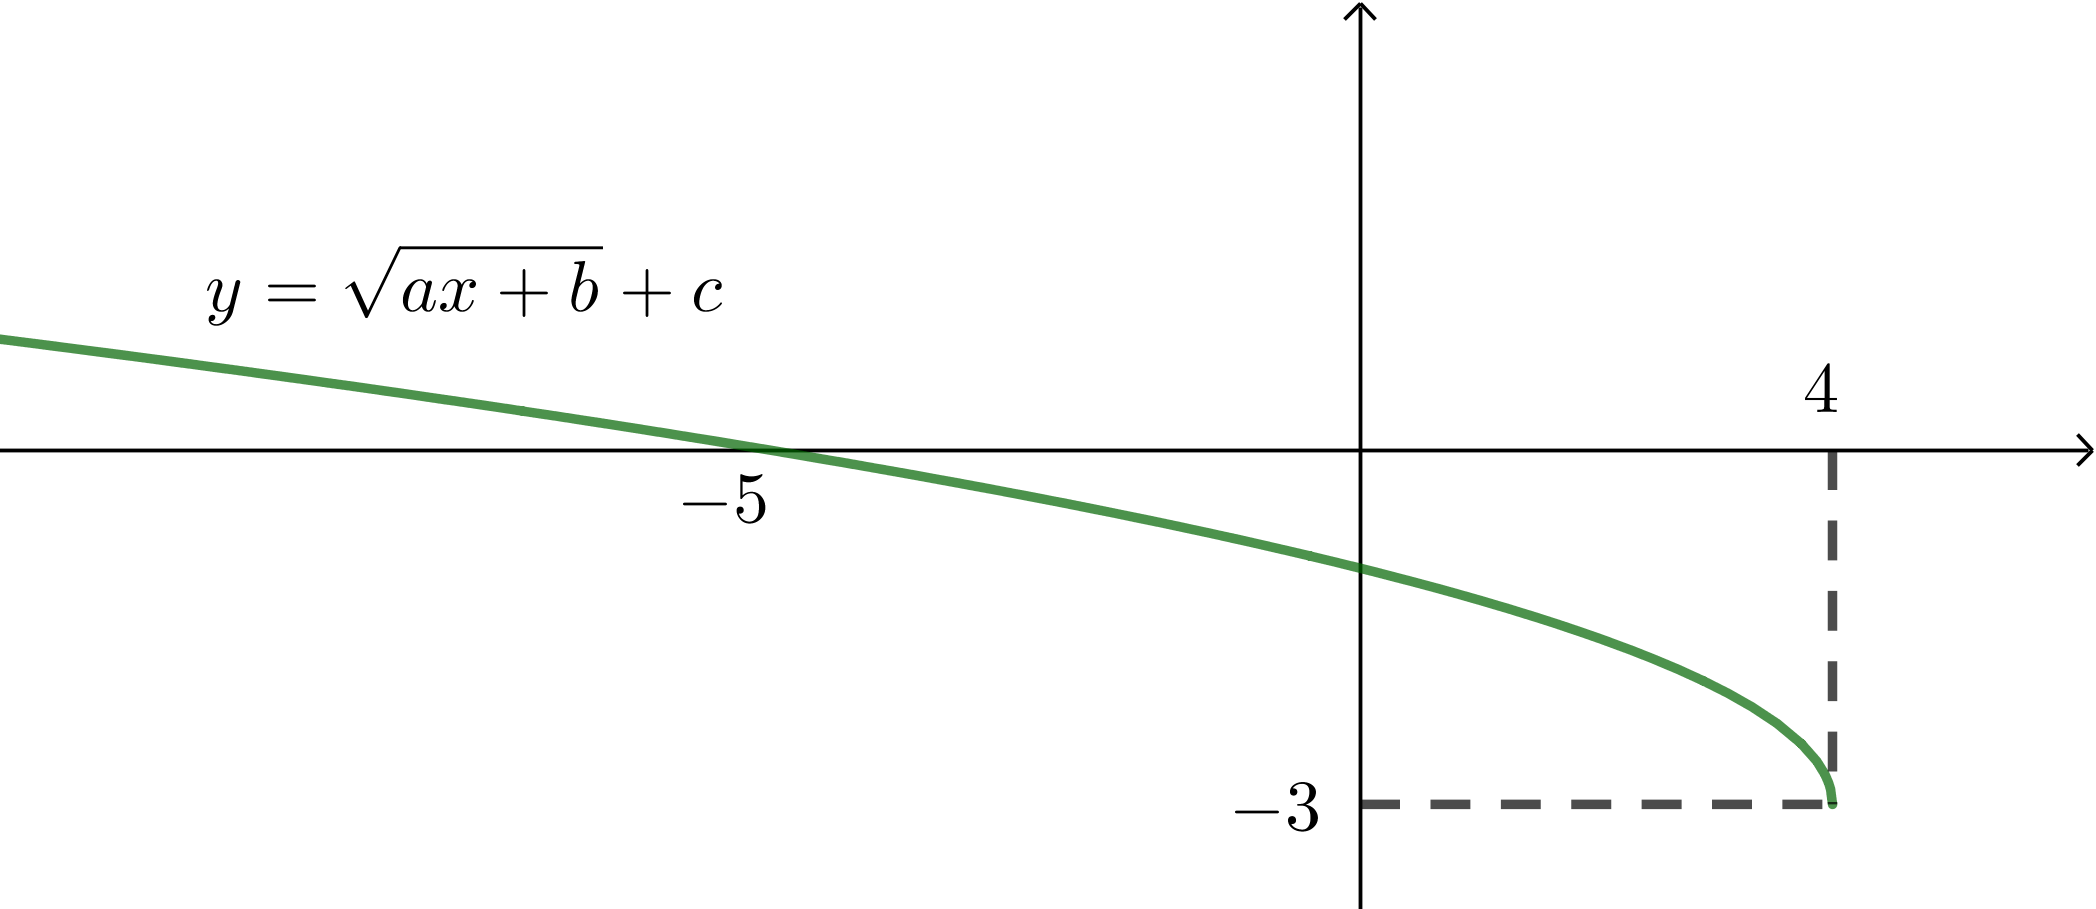
\includegraphics[width=0.5\textwidth]{irr}
\end{figure*}
\par\bigskip
\tabb{-10}{-8}{-6}{-4}{-2}

\clearpage
% 무리 8-4
\prob{}
\(-2\le x\le2\)에서 함수 \(y=4-\sqrt{5-2x}\)의 최댓값을 \(M\), 최솟값을 \(m\)이라고 할 때, \(M+m\)의 값은?
\par\bigskip
\tabb12345

% 무리 8-5
\prob{}
함수 \(y=\sqrt{x-2}\)의 그래프와 직선 \(y=x+k\)가 서로 다른 두 점에서 만나도록 하는 모든 실수 \(k\)의 값의 범위가 \(a\le k<b\)일 때, 두 상수 \(a\), \(b\)의 곱 \(ab\)의 값은?
\par\bigskip
\tabb{-\frac72}{-\frac34}1{\frac54}{\frac72}

% 무리 8-6
\prob{}
두 함수 \(y=\sqrt{x-1}+1\), \(y=x^2-2x+2\:(x\ge1)\)의 그래프가 두 점에서 만날 때, 이 두 점 사이의 거리는?
\par\bigskip
\tabb1{\sqrt2}{\sqrt3}2{\sqrt5}
\end{document}